% This LaTeX was auto-generated from MATLAB code.
% To make changes, update the MATLAB code and export to LaTeX again.

\documentclass{article}

\usepackage[utf8]{inputenc}
\usepackage[T1]{fontenc}
\usepackage{lmodern}
\usepackage{graphicx}
\usepackage{color}
\usepackage{listings}
\usepackage{hyperref}
\usepackage{amsmath}
\usepackage{amsfonts}
\usepackage{epstopdf}
\usepackage{matlab}

\sloppy
\epstopdfsetup{outdir=./}
\graphicspath{ {./ejercicio06_images/} }

\begin{document}

\matlabtitle{Ejercicio Nº6}


\begin{matlabcode}
clear;clc;
\end{matlabcode}

\matlabheading{Valores de los componentes}

\begin{matlabcode}
R1=1;
R2=1;
L1=2;
C1=1;
C2=1;

w=1;
\end{matlabcode}

\matlabheading{Condiciones iniciales}

\begin{matlabcode}
v01=0.5;
v02=0.5;
i01=0.5;
\end{matlabcode}

\matlabheading{Valores de tiempo y paso}

\begin{matlabcode}
ti=0;
tf=10;
h=0.001;
\end{matlabcode}

\matlabheading{Matrices de forma generalizadas}

\begin{matlabcode}
M=[C1 0 0;0 C2 0;0 0 L1]
\end{matlabcode}
\begin{matlaboutput}
M = 3x3    
     1     0     0
     0     1     0
     0     0     2

\end{matlaboutput}
\begin{matlabcode}
N=[1/R1 0 1;0 1/R2 -1;-1 1 0]
\end{matlabcode}
\begin{matlaboutput}
N = 3x3    
     1     0     1
     0     1    -1
    -1     1     0

\end{matlaboutput}
\begin{matlabcode}
Xant=[v01;v02;i01]
\end{matlabcode}
\begin{matlaboutput}
Xant = 3x1    
    0.5000
    0.5000
    0.5000

\end{matlaboutput}
\begin{matlabcode}
solu=[];
\end{matlabcode}

\matlabheading{Método Backward Euler}

\begin{matlabcode}
it=1;
for i= ti:h:tf
    %Fuente variable
    E(it,1)=awgn(0.5*sin(w*i),30);

    %Se calcula el valor de la matriz u para cada punto 
    B=[E(it,1)/R1;0;0];
    
    X=((((1/h).*M)+N)\B) + ((((1/h).*M)+N)\((1/h).*M)*Xant);
    
    solu=[solu X];
    Xant=X;
    it=it+1;
end
\end{matlabcode}

\vspace{1em}

\begin{matlabcode}
solu=solu';
\end{matlabcode}

\matlabheading{Gráfico}

\begin{matlabcode}
t=ti:h:tf;
plot(t,E,'-.m',t,solu(:,2),'-b')
title('Solución respuesta temporal');
xlabel('Tiempo [s]');
ylabel('Tensión [V]');
ylim([-0.7,0.7])
grid
\end{matlabcode}
\begin{center}
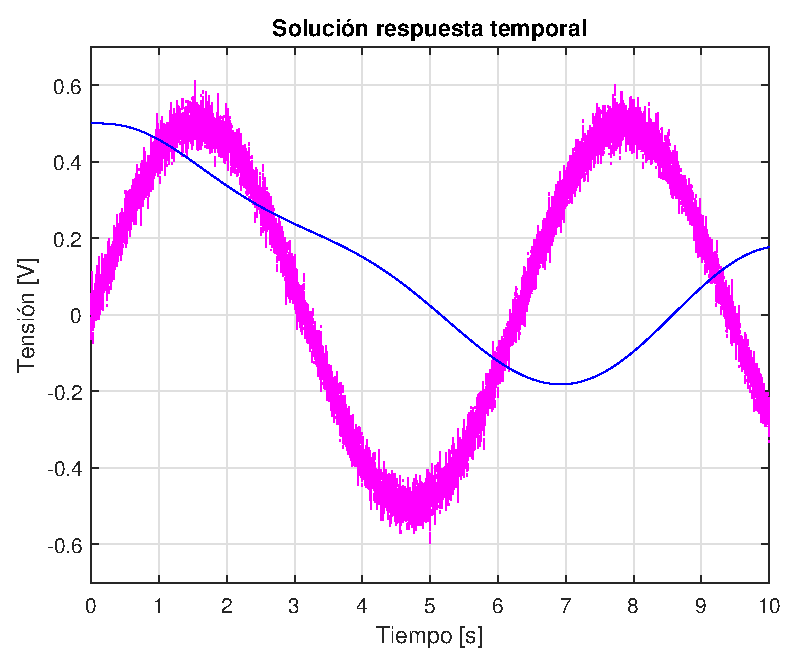
\includegraphics[width=\maxwidth{56.196688409433015em}]{figure_0_06}
\end{center}

\end{document}
